% last updated in April 2002 by Antje Endemann
% Based on CVPR 07 and LNCS, with modifications by DAF, AZ and elle, 2008 and AA, 2010, and CC, 2011; TT, 2014; AAS, 2016

\documentclass{llncs}
\usepackage{graphicx}
\usepackage{amsmath,amssymb} % define this before the line numbering.
\usepackage{ruler}
\usepackage{subcaption}
\captionsetup{compatibility=false}
\usepackage{xcolor}
\usepackage[width=122mm,left=12mm,paperwidth=146mm,height=193mm,top=12mm,paperheight=217mm]{geometry}
\usepackage{multirow}

\newcommand{\jason}[1]{\textcolor{orange}{\textbf{JASON: #1}}}
\newcommand{\madan}[1]{\textcolor{red}{#1}}


\begin{document}
% \renewcommand\thelinenumber{\color[rgb]{0.2,0.5,0.8}\normalfont\sffamily\scriptsize\arabic{linenumber}\color[rgb]{0,0,0}}
% \renewcommand\makeLineNumber {\hss\thelinenumber\ \hspace{6mm} \rlap{\hskip\textwidth\ \hspace{6.5mm}\thelinenumber}}
% \linenumbers
\pagestyle{headings}
\mainmatter
\def\ECCV18SubNumber{1816}  % Insert your submission number here

\title{TARP: Tensorflow-based Activity Recognition Platform} % Replace with your title

\titlerunning{TARP: Tensorflow-based Activity Recognition Platform}

\authorrunning{Eric Hofesmann, Madan Ravi Ganesh \and Jason J. Corso}

\author{Eric Hofesmann, Madan Ravi Ganesh \and Jason J. Corso}
\institute{University of Michigan}
\newcommand{\acro}{TARP}

\maketitle

\begin{abstract}
\keywords{}
\end{abstract}

\section{Introduction}
\label{sec:intro}

\section{Overview of \acro}
\label{sec:overview}

\begin{figure}[b!]
\centering
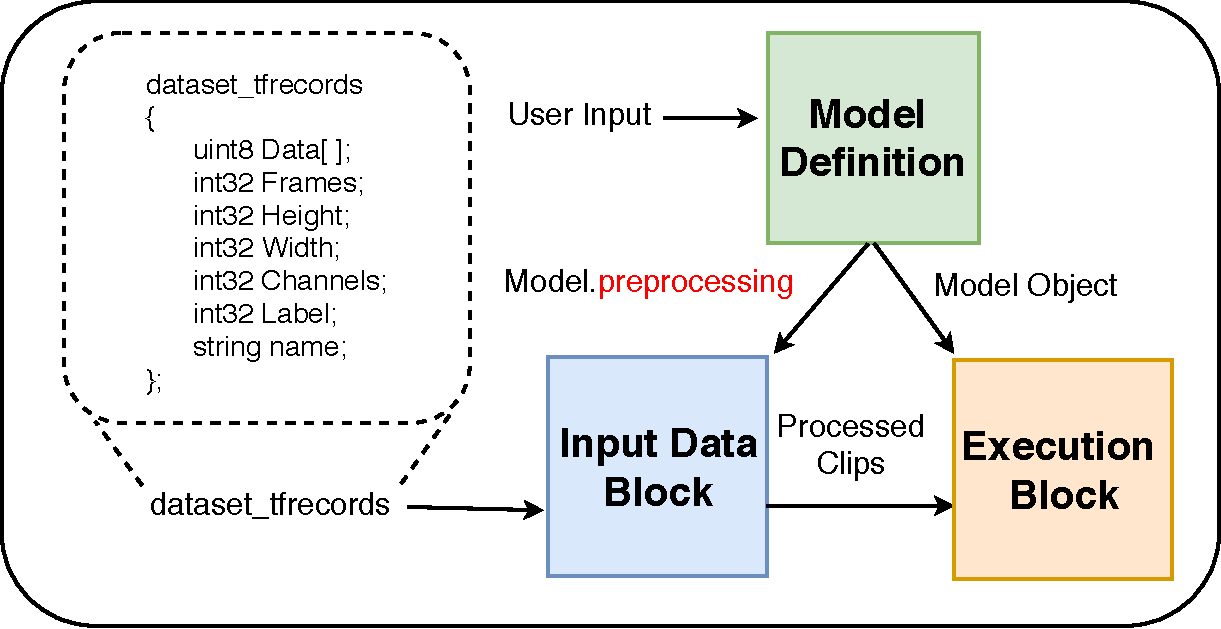
\includegraphics[width=0.8\textwidth]{images/overview.pdf}
\caption{Illustration of the two main components of \acro}
\label{fig:overview}
\end{figure}

\acro~comprises of two main components, 1) the data input block, and 2) the execution block, as shown in Fig.~\ref{fig:overview}. 
The pipeline contained within the data input block can be divided into three simple stages,
\begin{enumerate}
\item Read video data from disk
\item Extract the desired number of clips from a given video
\item Preprocess the frames of clips using a selected model's preprocessing strategy.
\end{enumerate}
The execution block houses all of the code required to setup, train, test as well as log the outputs of a chosen model.
This includes defining the layers that comprise the model, training the model up to a predetermined number of epochs, saving parameter values of a model are regular intervals and finally testing the performance of the trained model over a variety of recognition metrics.
The following sections provide an in depth discussion of the setup and structure of various components of the platform.

\section{Input Pipeline}
\label{sec:ippipeline}

\section{Execution Block}
\label{sec:execblock}

\begin{figure}[t!]
\centering
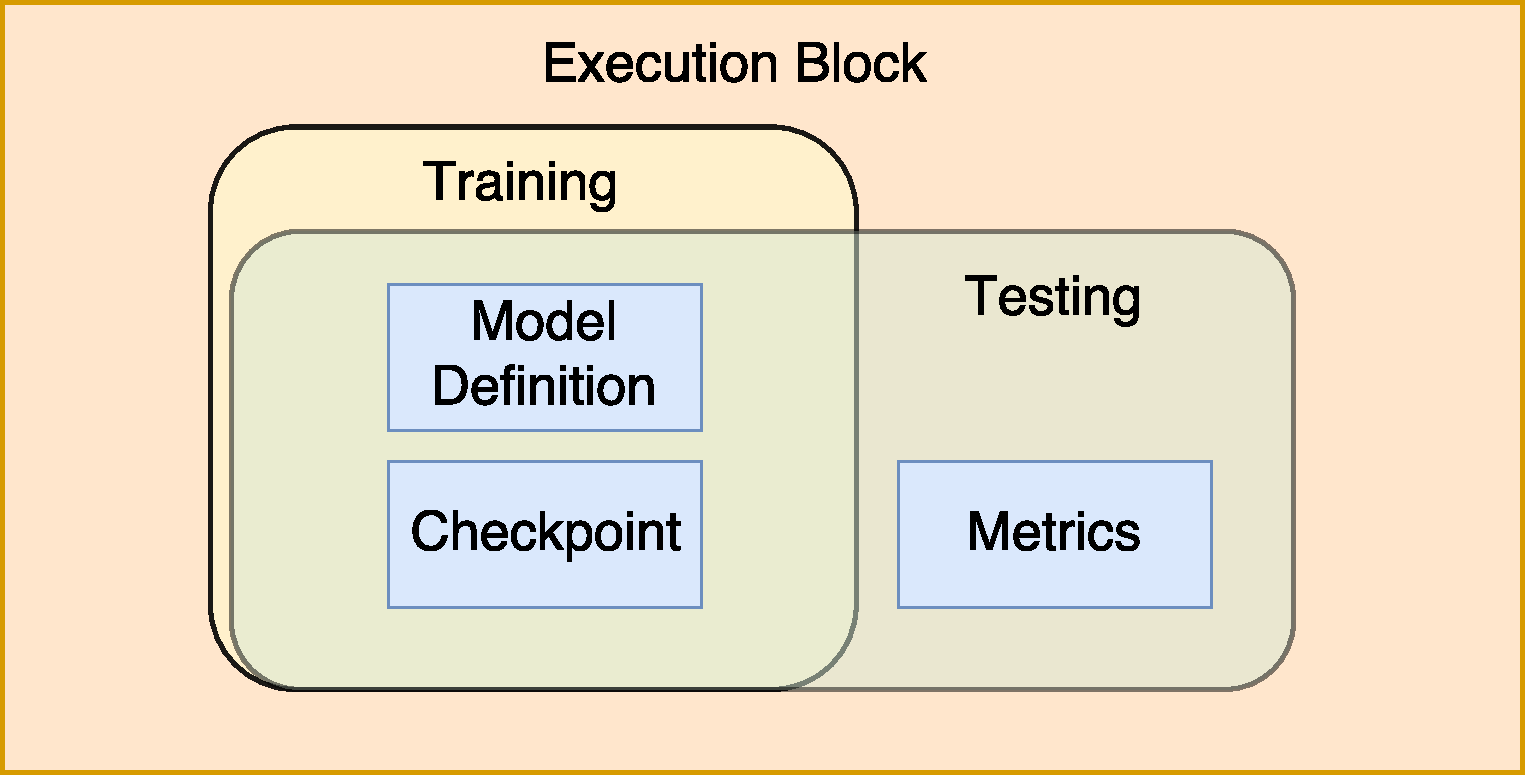
\includegraphics[width=0.8\columnwidth]{images/exec_block.pdf}
\caption{Training and Testing functions are the two major phases within the execution block. Model definitions and checkpoint-based functions are part of both training and testing functions while metrics are calculated after models are tested.}
\label{fig:exec_block}
\end{figure}

\subsection{Model Description}
\label{sec:modeldesc}

\subsection{Checkpoint}
\label{sec:checkpoint}

\subsection{Metrics}
\label{sec:metrics}

\clearpage

\bibliographystyle{splncs}
\bibliography{egbib}

\end{document}

\grid
\grid
\grid
\grid
\grid


